\subsection{Qualitative data}

Below, the most important results from the stakeholder and coach interviews are presented.

\subsubsection{Stakeholder interview findings: Entrepreneurship education considerations}
Through early interviews with YoungDrive staff, it is clear that YoungDrive's entrepreneurship education methodology goes hand in hand with the presented theory. It's mottos are: "Dream big, start small", "Learning by doing" and "We have fun!" \citep{youngdrive-manual}. The YoungDrive program seems to be very appreciated by every party, especially the project partner, Plan International. The interviews with Plan International (see figure \ref{fig:stakeholderInterview}) showed great knowledge about YoungDrive's positive effect on the youth.

\begin{figure}[h]
  \centering
  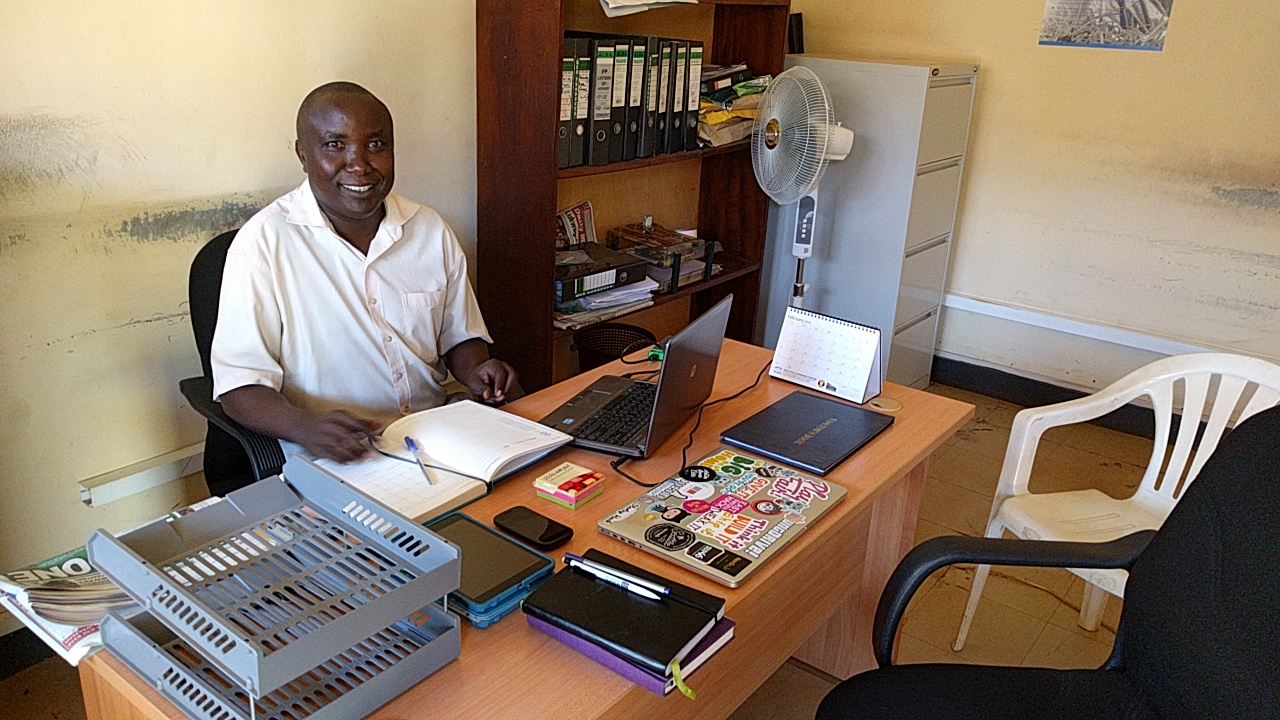
\includegraphics[width=0.8\textwidth]{iteration1/stakeholderInterview.jpg}
  \caption{Meeting with Plan from the office in Tororo, making final preparations for the meetings.}
  \label{fig:stakeholderInterview}
\end{figure}

Both in regards to designing for the users and for the above reason, the app should be a complement to YoundDrive's existing training material and the structure of the program.

A challenging part of the work is that YoungDrive consists of both the practical skills of the entrepreneur, theoretical material of running a business, and an entrepreneurial mindset. Therefore, both how to assess knowledge, and build habits, needs to be examined.

As the stakeholder interviews answered "What's it like being a coach?", their perspectives could now be understood and summed into a early understanding of the coach situation. The stakeholder interviews heavily informed the Questionnaire guide, highlighting aspects that had previously not been taken into account.

\subsubsection{Coach interview and field visit findings: Teaching with confidence}

The purpose of the coach interviews and observations was to understand "What's it like being a coach?", from the coaches own perspective. Thanks to having similar interviews with stakeholders, the coaches' opinions and experiences could be compared. Also, more detailed answers on background, desires, experience and situation could be provided.

 From the interviews and observations it was understood that CBTs can be responsible for from 7 up to 12 different youth groups in different programs, and such a high number places huge demands on the CBT. Even if there are only 7 groups, being behind on schedule or not being confident, can be very demanding.

%\textbf{Stayover at Patrick:} På morgonen visade Patrick mig hur han jobbar med deras tomt, var det odlas ris, och andra råvaror, deras djur, deras story från Syd-Sudan, till Kampala, till hyddan här i Tororo, och hans värderingar.

%Efter en ungdomssession nästföljande dag besökte vi och hälsade kort på en av de 2 CBT:s vi har session med idag. Sedan hade jag och Patrick den obligatoriska review av ungdoms-sessionen, och jag bjöd honom på middag. Kl. 19 ringde hans fru (som har börjat få tecken av malaria) och skyndade hem.

%Nästa ungdomssession fick jag besöka en annan CBT. Vi var tidiga. Sedan började jag prata med henne, och fick bra tillfälle att intervjua henne och även förklara för henne vad jag gjorde där. Det blev underligt att förklara för henne: Patrick påminde, när jag tabbat mig, att “Marcus, du måste förklara för X vad en app är”. Så hon fick låna min mobil, och jag förklarade att app var kort för applikation, och att för varje applikation har ett eget syfte, t.ex. ta foton. Jag bad henne klicka, svårt, råkade klicka åt henne, men sedan lät jag henne göra. Efter hon sett att det hon såg i skärmen var det hon såg på riktigt, blev hon jätteglad och började fundera vad hon skulle fota. Hon reste sig och gick runt hörnet, och jag följde efter. Hon fotade, efter att noggrannt tänkt igenom, att hon fotade buskarna med frukt. Sedan sade jag hon kunde fortsätta fota, och då tog hon ett litet runt hus utanför.

The interviews and observations with CBTs, Project Leaders and stakeholders led to the realization that different coaches handles this differently well. All coaches possess high self-confidence in varying degrees in various situations, and as a result, quality among coaches is unbalanced, which stakeholders see as a challenge. Depending on the situation, everything is going according to plan, you are not confident, or you are falling behind with the schedule, you can be in one of these three Need groups:

\begin{itemize}
  \item The ideal coach
  \item The realistic coach
  \item The challenged coach
\end{itemize}

It was discovered that coach confidence comes largely from being able to have good youth sessions, see figure \ref{youthSession1}. This is important, because according to the interviews, being a high-quality YoungDrive coach to a large extent means having high-quality youth sessions. For having a high-quality youth session, these are the most important attributes:

\begin{itemize}
  \item Correct information
  \item Correct structure
  \item Time management
  \item Fun atmosphere
\end{itemize}

\begin{figure}[h]
  \centering
  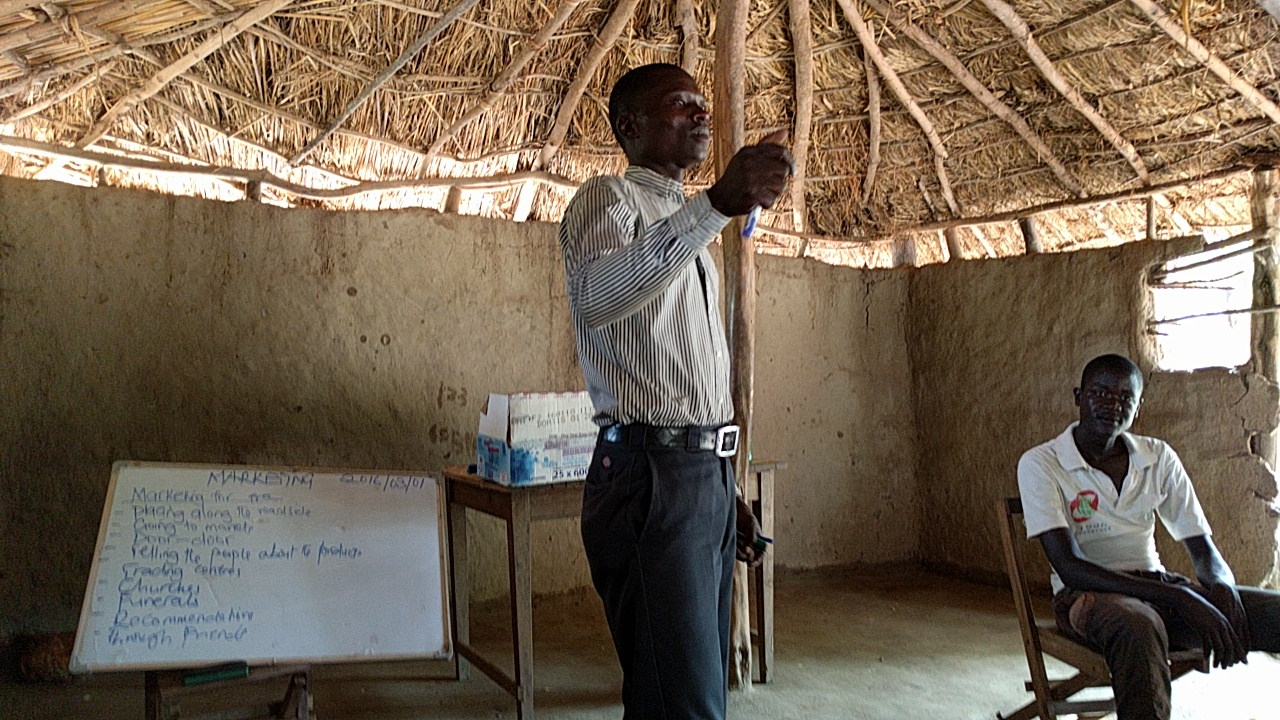
\includegraphics[width=0.8\textwidth]{iteration1/youthSession.jpg}
  \caption{Observing a youth session, the coach using the whiteboard to make certain concepts more clear.}
  \label{fig:youthSession1}
\end{figure}

These findings were used to inform the Customer Journey Map workshop. In addition to the findings here, questions were also asked around etnography.

